\documentclass{beamer}
\usepackage{ctex, hyperref}
\usepackage[T1]{fontenc}

% other packages
\usepackage{latexsym,amsmath,xcolor,multicol,booktabs,calligra,color}
\usepackage{graphicx,pstricks,listings,stackengine,subfigure}

\author{Can Xu}
\title{Self introduction and future plans}
\subtitle{}
\institute{}
\date{2023/6/17}
\usepackage{zjgsu}
\setsansfont{Times New Roman}
\setmainfont{Times New Roman}

% defs
\def\cmd#1{\texttt{\color{red}\footnotesize $\backslash$#1}}
\def\env#1{\texttt{\color{blue}\footnotesize #1}}
\definecolor{deepblue}{rgb}{0,0,0.5}
\definecolor{deepred}{rgb}{0.6,0,0}
\definecolor{deepgreen}{rgb}{0,0.5,0}
\definecolor{halfgray}{gray}{0.55}

\lstset{
    basicstyle=\ttfamily\small,
    keywordstyle=\bfseries\color{deepblue},
    emphstyle=\ttfamily\color{deepred},    % Custom highlighting style
    stringstyle=\color{deepgreen},
    numbers=left,
    numberstyle=\small\color{halfgray},
    rulesepcolor=\color{red!20!green!20!blue!20},
    frame=shadowbox,
}


\begin{document}

\kaishu
\begin{frame}
    \titlepage
    \centering{}
    % \begin{figure}[htpb]
    %     \begin{center}
    %         
\includegraphics[width=0.15\linewidth]{figure/zjgsu} % 这个位置可能需要调整
    %     \end{center}
    % \end{figure}
\end{frame}

\begin{frame}
    \tableofcontents[sectionstyle=show,subsectionstyle=show/shaded/hide,subsubsectionstyle=show/shaded/hide]
\end{frame}

\section{Basic information}
\begin{frame}{Basic information}
    \begin{itemize}
        \item I'm from Suzhou, Jiangsu.
        \item I got my bachelor's degree at Nanjing University of Information Science \& Technology and currently a master degree candidate of science in Zhejiang Gongshang University.
        \item My github page is \url{https://github.com/LEOXC1571} and my personal blog is \url{https://leoxc1571.github.io/}
    \end{itemize}
\end{frame}

\section{Publications}
\begin{frame}{A fairness-aware graph contrastive learning recommender framework for social tagging systems}
    \begin{itemize}
        \item The proposed method integrates contrastive learning into tag-aware recommender systems. By perturbing features with normalized noises, different perspectives on features are generated. They help the model learn high quality features via contrastive learning tasks.
        \item In order to promote fairness of recommendations, we introduce fairness-aware learning, which jointly optimizes TAGCL through negative tag loss and TransT regularization. Negative tag loss leverages the distribution difference between items and tags in the training data.
        \item TransT regularization is also propsosed to promote consistency between two bipartite graphs. The differences between tag embeddings in separate graphs are regarded as relations between users and items.
    \end{itemize}
\end{frame}

\begin{frame}{A fairness-aware graph contrastive learning recommender framework for social tagging systems}
    \begin{figure}[H]
        \centering
        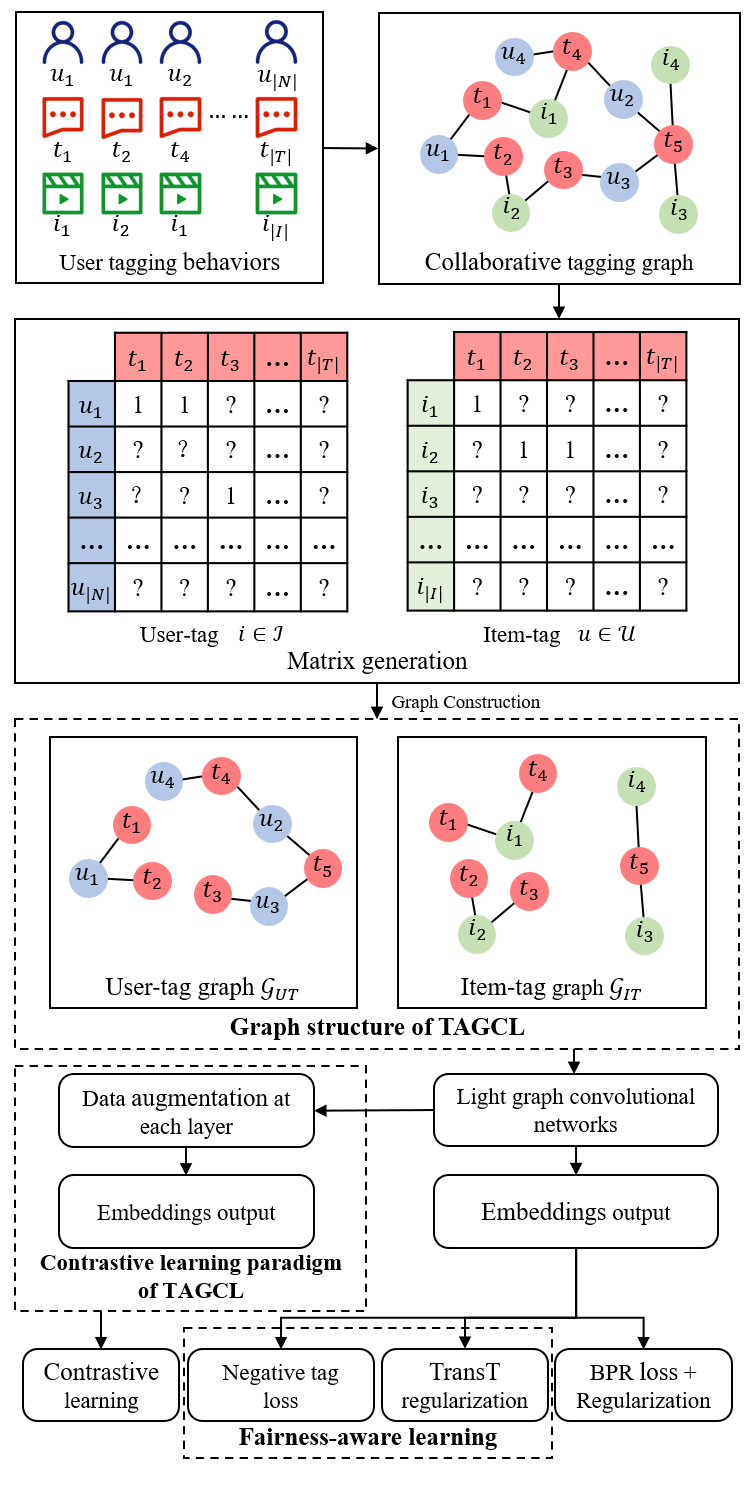
\includegraphics[width=0.28\linewidth]{figure/tagcl.png}
        \caption{Overall structure of TAGCL}
    \end{figure}
\end{frame}

\begin{frame}{A fairness-aware graph contrastive learning recommender framework for social tagging systems}
    \begin{figure}[H]
        \centering
        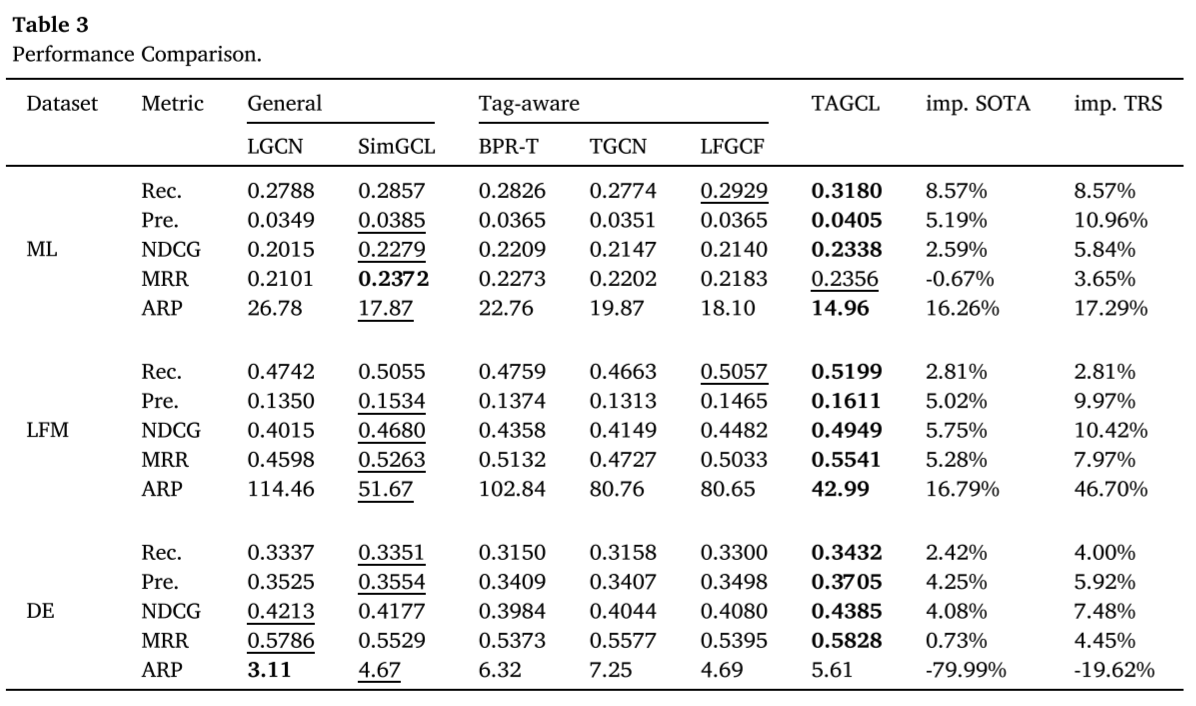
\includegraphics[width=\linewidth]{figure/tagcl_performance.png}
    \end{figure}
\end{frame}

\begin{frame}{Pursuit and Evasion Strategy of a Differential Game Based on Deep Reinforcement Learning}
    \begin{itemize}
        \item For the kinematic solve of dog sheep game, by finding the equilibrium point in the game, this study successfully establishes the kinematic pursuit and evasion policies.
        \item Leverage DQN and DDPG models to train the escaping strategy for intelligent agent.
        \item Propose a refined reward mechanism and an attenuation mechanism to minimize the defect of DQN.
    \end{itemize}
\end{frame}


% \begin{frame}{为什么需要Beamer}
%     \begin{itemize}[<+-| alert@+>] % 当然,除了alert,手动在里面插 \pause 也行
%         \item 大家都会\LaTeX{},好多学校都有自己的Beamer主题
%         \item 中文支持请选择 Xe\LaTeX{} 编译选项
%         \item Overleaf项目地址位于 \url{https://www.overleaf.com/latex/templates/thu-beamer-theme/vwnqmzndvwyb},可以直接使用
%         \item GitHub项目地址位于 \url{https://github.com/Trinkle23897/THU-Beamer-Theme},如果有bug或者feature request可以去里面提issue
%     \end{itemize}
% \end{frame}


\section{Experiences}
\begin{frame}{Internship at Zhejiang Lab}
    \begin{itemize}
        \item 生成模型近年来在作画、视频创作、空间建模、文本生成等多方面都有了成功的应用。早期的生成模型研究主要集中在变分自编码器(VAE)、生成对抗网络(GAN)、流型模型(Flow-based models)、自回归模型(Auto-regressive models)及深度强化学习领域。近两年来,基于扩散模型的生成模型(Diffusion-based models)以其优异的性能、计算资源消耗相对较少在学术圈与工业界爆火。
        \item 相关Diffusion模型的研究包括对干扰、去噪过程的改进(DDPMs,SGMs,Score SDEs),采样策略的改进,损失函数,各类型数据应用(计算机视觉、自然语言处理、时序建模、信号传递、多模态学习、图建模、医学影像)等。
    \end{itemize}
\end{frame}

\begin{frame}{计算医药}
    \begin{itemize}
        \item 生成模型的发展也带动了其在智能计算领域的应用。5年前,药物分子、蛋白质配体分子等分子学习任务主要聚焦于2D分子结构,但实际上,分子结构信息远不止原子间的拓扑结构信息这么简单,因此某一分子在自然界中可能存在种类繁多的同分异构体,故近来对分子的研究拓展到了结合3D信息对不同分子构型的相关研究。因此在3D分子生成任务上,目标不再是生成简单的可能有效的分子,更要生成具备理想属性和性质稳定的分子3D构型。
        \item 3D分子生成任务又可分为3D构型生成与全新分子生成。3D构型生成的目标是根据给定的分子式,生成理想的三维构型。全新分子生成的目标则是凭空生成全新的、有效的分子。
        \item 3D构型生成的研究有基于VAE的CVGAE,GraphDG,ConfVAE,基于扩散模型的ConfGF,EVFN,GeoDiff等。
    \end{itemize}
\end{frame}


\section{研究内容}
\begin{frame}{前期准备}
    \begin{itemize}
        \item \textcolor[rgb]{0.827,0.318,0.298}{本文意在利用生成模型,提出创新的算法,生成全新且有效的分子。}
        \item 本文首先选取GEOM-QM9和GEOM-Drugs作为研究数据集。GEOM-QM9包含130831个分子,平均每个分子由19个分子构成。
        \item GEOM-Drugs包含超过600W个分子构型,将每个分子的不同构型经过筛选后,处理得到29W个稳定的分子构型,平均每个分子由44个原子构成。
    \end{itemize}
\end{frame}

\begin{frame}{生成模型构建}
    \begin{itemize}
        \item 本文基于DDPMs构建分子生成模型框架,包括扩散过程与去噪过程。
        \item 扩散过程本质是通过给初始数据有规律地增加噪声,使其经过$T$时间步后收敛至高斯噪声。
        \item 去噪过程的本质是通过设计的去噪神经网络内核,将高斯噪声还原至初始状态,使其与初始数据相似。
    \end{itemize}
\end{frame}



\section{计划进度}
\begin{frame}
    \begin{itemize}
        \item 2023.01-2023.03:前期调研与相关文献阅读
        \item 2023.03-2023.04:模型搭建
        \item 2023.04-2023.05:模型训练,性能调优与对比试验
        \item 2023.05-2023.07:文章撰写
        \item 2023.07-2023.09:文章修改
    \end{itemize}
\end{frame}

% \begin{frame}{这一份主题目前与THU Beamer Theme区别在于}
%     \begin{itemize}
%         \item 修改校徽
%         \item 修改主题色
%     \end{itemize}
% \end{frame}

% \begin{frame}{Why Beamer}
%     \begin{itemize}
%         \item \LaTeX 广泛用于学术界,期刊会议论文模板
%     \end{itemize}
%     \begin{table}[h]
%         \centering
%         \begin{tabular}{c|c}
%             Microsoft\textsuperscript{\textregistered}  Word & \LaTeX \\
%             \hline
%             文字处理工具 & 专业排版软件 \\
%             容易上手,简单直观 & 容易上手 \\
%             所见即所得 & 所见即所想,所想即所得 \\
%             高级功能不易掌握 & 进阶难,但一般用不到 \\
%             处理长文档需要丰富经验 & 和短文档处理基本无异 \\
%             花费大量时间调格式 & 无需担心格式,专心作者内容 \\
%             公式排版差强人意 & 尤其擅长公式排版 \\
%             二进制格式,兼容性差 & 文本文件,易读、稳定 \\
%             付费商业许可 & 自由免费使用 \\
%         \end{tabular}
%     \end{table}
% \end{frame}

% \begin{frame}{排版举例}
%     \begin{exampleblock}{无编号公式} % 加 * 
%         \begin{equation*}
%             J(\theta) = \mathbb{E}_{\pi_\theta}[G_t] = \sum_{s\in\mathcal{S}} d^\pi (s)V^\pi(s)=\sum_{s\in\mathcal{S}} d^\pi(s)\sum_{a\in\mathcal{A}}\pi_\theta(a|s)Q^\pi(s,a)
%         \end{equation*}
%     \end{exampleblock}
%     \begin{exampleblock}{多行多列公式\footnote{如果公式中有文字出现,请用 $\backslash$mathrm\{\} 或者 $\backslash$text\{\} 包含,不然就会变成 $clip$,在公式里看起来比 $\mathrm{clip}$ 丑非常多。}}
%         % 使用 & 分隔
%         \begin{align}
%             Q_\mathrm{target}&=r+\gamma Q^\pi(s^\prime, \pi_\theta(s^\prime)+\epsilon)\\
%             \epsilon&\sim\mathrm{clip}(\mathcal{N}(0, \sigma), -c, c)\nonumber
%         \end{align}
%     \end{exampleblock}
% \end{frame}

% \begin{frame}
%     \begin{exampleblock}{编号多行公式}
%         % Taken from Mathmode.tex
%         \begin{multline}
%             A=\lim_{n\rightarrow\infty}\Delta x\left(a^{2}+\left(a^{2}+2a\Delta x+\left(\Delta x\right)^{2}\right)\right.\label{eq:reset}\\
%             +\left(a^{2}+2\cdot2a\Delta x+2^{2}\left(\Delta x\right)^{2}\right)\\
%             +\left(a^{2}+2\cdot3a\Delta x+3^{2}\left(\Delta x\right)^{2}\right)\\
%             +\ldots\\
%             \left.+\left(a^{2}+2\cdot(n-1)a\Delta x+(n-1)^{2}\left(\Delta x\right)^{2}\right)\right)\\
%             =\frac{1}{3}\left(b^{3}-a^{3}\right)
%         \end{multline}
%     \end{exampleblock}
% \end{frame}

% \begin{frame}{图形与分栏}
%     % From thuthesis user guide.
%     \begin{minipage}[c]{0.3\linewidth}
%         \psset{unit=0.8cm}
%         \begin{pspicture}(-1.75,-3)(3.25,4)
%             \psline[linewidth=0.25pt](0,0)(0,4)
%             \rput[tl]{0}(0.2,2){$\vec e_z$}
%             \rput[tr]{0}(-0.9,1.4){$\vec e$}
%             \rput[tl]{0}(2.8,-1.1){$\vec C_{ptm{ext}}$}
%             \rput[br]{0}(-0.3,2.1){$\theta$}
%             \rput{25}(0,0){%
%             \psframe[fillstyle=solid,fillcolor=lightgray,linewidth=.8pt](-0.1,-3.2)(0.1,0)}
%             \rput{25}(0,0){%
%             \psellipse[fillstyle=solid,fillcolor=yellow,linewidth=3pt](0,0)(1.5,0.5)}
%             \rput{25}(0,0){%
%             \psframe[fillstyle=solid,fillcolor=lightgray,linewidth=.8pt](-0.1,0)(0.1,3.2)}
%             \rput{25}(0,0){\psline[linecolor=red,linewidth=1.5pt]{->}(0,0)(0.,2)}
% %           \psRotation{0}(0,3.5){$\dot\phi$}
% %           \psRotation{25}(-1.2,2.6){$\dot\psi$}
%             \psline[linecolor=red,linewidth=1.25pt]{->}(0,0)(0,2)
%             \psline[linecolor=red,linewidth=1.25pt]{->}(0,0)(3,-1)
%             \psline[linecolor=red,linewidth=1.25pt]{->}(0,0)(2.85,-0.95)
%             \psarc{->}{2.1}{90}{112.5}
%             \rput[bl](.1,.01){C}
%         \end{pspicture}
%     \end{minipage}\hspace{1cm}
%     \begin{minipage}{0.5\linewidth}
%         \medskip
%         %\hspace{2cm}
%         \begin{figure}[h]
%             \centering
%             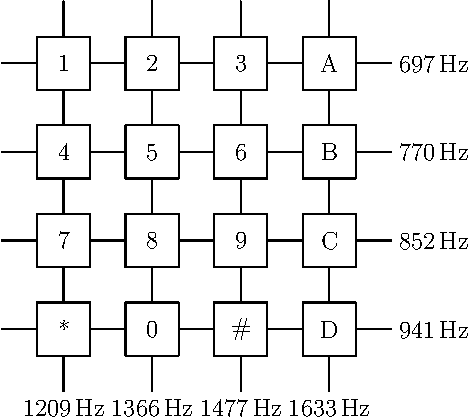
\includegraphics[height=.4\textheight]{figure/dtmf.pdf}
%         \end{figure}
%     \end{minipage}
% \end{frame}

% \begin{frame}[fragile]{\LaTeX{} 常用命令}
%     \begin{exampleblock}{命令}
%         \centering
%         \footnotesize
%         \begin{tabular}{llll}
%             \cmd{chapter} & \cmd{section} & \cmd{subsection} & \cmd{paragraph} \\
%             章 & 节 & 小节 & 带题头段落 \\\hline
%             \cmd{centering} & \cmd{emph} & \cmd{verb} & \cmd{url} \\
%             居中对齐 & 强调 & 原样输出 & 超链接 \\\hline
%             \cmd{footnote} & \cmd{item} & \cmd{caption} & \cmd{includegraphics} \\
%             脚注 & 列表条目 & 标题 & 插入图片 \\\hline
%             \cmd{label} & \cmd{cite} & \cmd{ref} \\
%             标号 & 引用参考文献 & 引用图表公式等\\\hline
%         \end{tabular}
%     \end{exampleblock}
%     \begin{exampleblock}{环境}
%         \centering
%         \footnotesize
%         \begin{tabular}{lll}
%             \env{table} & \env{figure} & \env{equation}\\
%             表格 & 图片 & 公式 \\\hline
%             \env{itemize} & \env{enumerate} & \env{description}\\
%             无编号列表 & 编号列表 & 描述 \\\hline
%         \end{tabular}
%     \end{exampleblock}
% \end{frame}

% \begin{frame}[fragile]{\LaTeX{} 环境命令举例}
%     \begin{minipage}{0.5\linewidth}
% \begin{lstlisting}[language=TeX]
% \begin{itemize}
%   \item A \item B
%   \item C
%   \begin{itemize}
%     \item C-1
%   \end{itemize}
% \end{itemize}
% \end{lstlisting}
%     \end{minipage}\hspace{1cm}
%     \begin{minipage}{0.3\linewidth}
%         \begin{itemize}
%             \item A
%             \item B
%             \item C
%             \begin{itemize}
%                 \item C-1
%             \end{itemize}
%         \end{itemize}
%     \end{minipage}
%     \medskip
%     \pause
%     \begin{minipage}{0.5\linewidth}
% \begin{lstlisting}[language=TeX]
% \begin{enumerate}
%   \item 巨佬 \item 大佬
%   \item 萌新
%   \begin{itemize}
%     \item[n+e] 瑟瑟发抖
%   \end{itemize}
% \end{enumerate}
% \end{lstlisting}
%     \end{minipage}\hspace{1cm}
%     \begin{minipage}{0.3\linewidth}
%         \begin{enumerate}
%             \item 巨佬
%             \item 大佬
%             \item 萌新
%             \begin{itemize}
%                 \item[n+e] 瑟瑟发抖
%             \end{itemize}
%         \end{enumerate}
%     \end{minipage}
% \end{frame}

% \begin{frame}[fragile]{\LaTeX{} 数学公式}
%     \begin{columns}
%         \begin{column}{.55\textwidth}
% \begin{lstlisting}[language=TeX]
% $V = \frac{4}{3}\pi r^3$

% \[
%   V = \frac{4}{3}\pi r^3
% \]

% \begin{equation}
%   \label{eq:vsphere}
%   V = \frac{4}{3}\pi r^3
% \end{equation}
% \end{lstlisting}
%         \end{column}
%         \begin{column}{.4\textwidth}
%             $V = \frac{4}{3}\pi r^3$
%             \[
%                 V = \frac{4}{3}\pi r^3
%             \]
%             \begin{equation}
%                 \label{eq:vsphere}
%                 V = \frac{4}{3}\pi r^3
%             \end{equation}
%         \end{column}
%     \end{columns}
%     \begin{itemize}
%         \item 更多内容请看 \href{https://zh.wikipedia.org/wiki/Help:数学公式}{\color{purple}{这里}}
%     \end{itemize}
% \end{frame}

% \begin{frame}[fragile]
%     \begin{columns}
%         \column{.6\textwidth}
% \begin{lstlisting}[language=TeX]
%     \begin{table}[htbp]
%       \caption{编号与含义}
%       \label{tab:number}
%       \centering
%       \begin{tabular}{cl}
%         \toprule
%         编号 & 含义 \\
%         \midrule
%         1 & 4.0 \\
%         2 & 3.7 \\
%         \bottomrule
%       \end{tabular}
%     \end{table}
%     公式~(\ref{eq:vsphere}) 的
%     编号与含义请参见
%     表~\ref{tab:number}。
% \end{lstlisting}
%         \column{.4\textwidth}
%         \begin{table}[htpb]
%             \centering
%             \caption{编号与含义}
%             \label{tab:number}
%             \begin{tabular}{cl}\toprule
%                 编号 & 含义 \\\midrule
%                 1 & 4.0\\
%                 2 & 3.7\\\bottomrule
%             \end{tabular}
%         \end{table}
%         \normalsize 公式~(\ref{eq:vsphere})的编号与含义请参见表~\ref{tab:number}。
%     \end{columns}
% \end{frame}

% \begin{frame}{作图}
%     \begin{itemize}
%         \item 矢量图 eps, ps, pdf
%         \begin{itemize}
%             \item METAPOST, pstricks, pgf $\ldots$
%             \item Xfig, Dia, Visio, Inkscape $\ldots$
%             \item Matlab / Excel 等保存为 pdf
%         \end{itemize}
%         \item 标量图 png, jpg, tiff $\ldots$
%         \begin{itemize}
%             \item 提高清晰度,避免发虚
%             \item 应尽量避免使用
%         \end{itemize}
%     \end{itemize}
%     \begin{figure}[htpb]
%         \centering
%         
\includegraphics[width=0.2\linewidth]{figure/zjgsu.jpg}
%         \caption{这个校徽就是矢量图}
%     \end{figure}
% \end{frame}





\begin{frame}
    \begin{center}
        {\Huge\calligra Thanks!}
    \end{center}
\end{frame}

\end{document}